\section{Implementation}
\label{sec:impl}

In this section, we describe how to evaluate \lang programs. First, we
generalize semi-naive evaluation to support lattices. We validate that our
implementation of semi-naive evaluation results in significant performance gains
and is competitive with the traditional set-only semi-naive evaluation
scheme in Bud. We also describe how we extended Bud to support \lang
with relatively few changes.

%\ifbool{socc-print-version}{\pagebreak}{}
\subsection{Evaluation Strategy}
\label{sec:lattice-eval-strat}
\emph{Naive} evaluation is a simple but inefficient approach to evaluating
recursive Datalog programs. Evaluation proceeds in rounds. In each round,
every rule in the program is evaluated over the entire database, including all
derivations made in previous rounds. This process stops when a round makes no
new derivations. Naive evaluation is inefficient because it makes many redundant
derivations: once a fact has been derived in round $i$, it is rederived in every
round $>i$.

\emph{Semi-naive} evaluation improves upon naive evaluation by making fewer
redundant derivations~\cite{Balbin1987}. Let $\Delta_0$ represent the initial
database state. In the first round, all the rules are evaluated over $\Delta_0$;
let $\Delta_1$ represent the new facts derived in this round. In the second
round, we only need to compute derivations that depend on $\Delta_1$ because
everything that can be derived purely from $\Delta_0$ has already been computed.

A similar evaluation strategy works for \lang statements that use lattice
morphisms. For a given lattice identifier $l$, let $\Delta_l^0$ represent the
lattice element associated with $l$ at the start of the current timestep. Let
$\Delta^r_l$ represent the new derivations for $l$ that have been made in
evaluation round $r$. During round one, the program's statements are evaluated
and $l$ is mapped to $\Delta_l^0$; this computes $\Delta^1_l$. In round two, $l$
is now mapped to $\Delta^1_l$ and evaluating the program's statements yields
$\Delta^2_l$. This process continues until $\Delta^i_l = \Delta^{i+1}_l$ for all
identifiers $l$.  The final value for $l$ is given by $\bigsqcup_{l: j=0}^i
\Delta^j_l$.

This optimization cannot be used for monotone functions that are not
morphisms. This is because semi-naive evaluation requires that we apply
functions to the partial results derived in each round $k$ into $\Delta_l^k$,
and later combine them using the lattice's merge operation---effectively
distributing the function across the merge.  For example, consider computing the
\texttt{lset} lattice's \texttt{size} method, which returns an \texttt{lmax}
lattice. The semi-naive strategy would compute
$\bigsqcup_{\mathtt{lmax}:j=0}^i size(\Delta^j_{\mathtt{lset}})$---the maximum of
the sizes of the incremental results produced in each round.  Thus it produces a
different result than naive evaluation, which evaluates the \texttt{size}
function against the complete database state in each round.

Implementing semi-naive style evaluation for lattices was straightforward. For
each lattice identifier $l$, we record two values: a ``total'' value (the least
upper bound of the derivations made for $l$ in all previous rounds) and a
``delta'' value (the least upper bound of the derivations made for $l$ in the
last round). We implemented a program rewrite that examines each \lang
statement. If a statement only applies morphisms to lattice elements, the
rewrite adjusts the statement to use the lattice's delta value rather than its
total value.

\subsection{Performance Validation}
\label{sec:lattice-perf}

\begin{figure}[t]
\centering
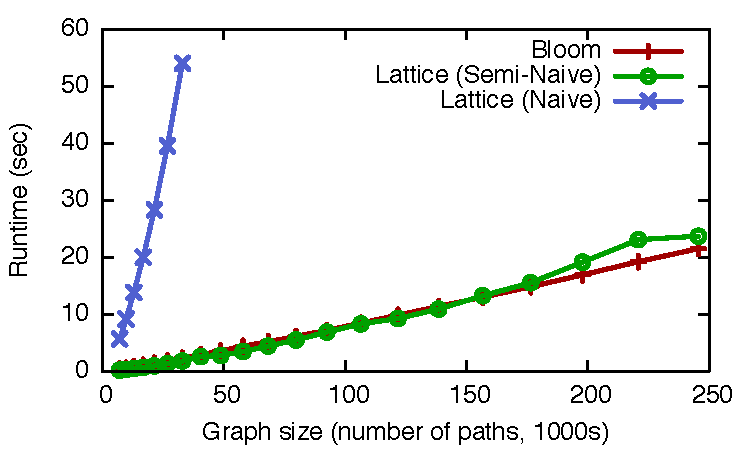
\includegraphics[width=\linewidth]{fig/sn_perf}
\caption{Performance of three different methods for computing the
  transitive closure of a graph.}
\label{fig:tc-perf-graph}
\end{figure}

To validate the effectiveness of semi-naive evaluation for \lang programs, we
wrote two versions of a program to compute the transitive closure of a directed
acyclic graph. One version was written in Bloom and used Bloom collections. The
other version was written in \lang using morphisms over the \texttt{lset}
lattice. For the \lang version, we ran the program both with and without
semi-naive evaluation enabled. As input, we generated synthetic graphs of
various sizes---in a graph with $n$ nodes, each node had roughly $\log_2 n$ outgoing
edges. We ran the experiment using a 2.13 GHz Intel Core 2 Duo processor and 4GB
of RAM, running Mac OS X 10.7.4 and Ruby 1.9.3-p194. We ran each program variant
five times on each graph and report the mean elapsed wall-clock time.

Figure~\ref{fig:tc-perf-graph} shows how the runtime of each program varied with
the size of the graph. Note that we only report results for the naive \lang
strategy on small input sizes because this variant ran very slowly as the graph
size increased. The poor performance of naive evaluation is not surprising:
after deriving all paths of length $n$, naive evaluation will then rederive all
those paths at every subsequent round of the fixpoint computation. In contrast,
after computing length $n$ paths, a semi-naive strategy will only generate
length $n+1$ paths in the next round. Bloom and semi-naive \lang achieve similar
results. We instrumented Bud to count the number of derivations made by the
Bloom and semi-naive lattice variants---as expected, both programs made a
similar number of derivations. These results suggest that our implementation of
semi-naive evaluation for \lang is effective and performs comparably with
a traditional implementation of semi-naive evaluation for sets.

For large inputs, Bloom began to outperform the semi-naive lattice variant. We
suspect this is because the lattice implementation copies more data than Bloom
does for this benchmark. Lattice elements are immutable, so the \texttt{lset}
merge function allocates a new object to hold the result of the merge. In
contrast, Bloom collections are modified in-place. We plan to improve the
lattice runtime to avoid copies when it can determine that in-place updates are
safe.

\subsection{Discussion}
When designing \lang, we chose to extend the original Bloom language rather than
inventing a new language from scratch. This design philosophy also applied to our
language implementation: we found we were able to to extend Bud to support \lang
with relatively minor changes.

Bud initially had about 7300 lines of Ruby source code (LOC). Adding support for
\lang required less than 1000 lines of added or modified code; moreover, most of
these changes were cleanly separated from the core Bud code. For example, the
built-in lattice types constituted 300 LOC and support for lattice-based query
plan elements required 250 LOC. In contrast, we had to make no changes to Bud's
core fixpoint loop and extending CALM analysis to support lattices required
modifying only 10 LOC. This experience suggests that support for lattices can be
added to an existing Datalog engine in a relatively straightforward manner.

%  300
% LOC were needed for the built-in lattice types and 200 LOC were required to
% provide

%  The core lattice
% features (the \texttt{Bud::Lattice} base class and the mapping from identifiers
% to lattice elements) required about 300 LOC; an additional 200 LOC was needed to
% implement lattice-based query plan elements. Notably, no changes were required
% to Bud's core fixpoint loop, while the program rewriting required to enable
% semi-naive evaluation only required 50 LOC.  Modifying Bud's collection classes
% to support merging of embedded lattice values required adding or modifying about
% 125 LOC. Extending CALM analysis to include lattices required modifying about 10
% LOC. The built-in lattice classes constituted an additional 300 LOC. In total,
% adding support for \lang required less than 1000 lines of added or modified
% code and took about three person-months of engineering time. This experience
% suggests that support for lattices can be added to an existing Datalog engine in
% a relatively straightforward manner.
